% ============================================================
% Verbesserungen gegenüber der Originalskizze:
%  1. Satellitenpositionen S1/S2 liegen jetzt exakt auf der
%     Ellipse (vorher: leicht ausserhalb bzw. innerhalb).
%  2. Die Flächen A1/A2 sind jetzt echte elliptische Sektoren
%     (Polygon entlang der Ellipsenkurve), keine Kreisbogen-
%     Näherung mehr. Weiterhin schematisch gleich gross
%     dargestellt (physikalisch exakt gleiche Flächen hätten
%     bei dieser Exzentrizität e=0.8 einen sehr grossen
%     Öffnungswinkel nahe der Terre zur Folge, was für eine
%     Prüfungsskizze unübersichtlich wäre).
%  3. Geschwindigkeitspfeile zeigen jetzt in die tatsächliche
%     Bahntangente (konsistente Umlaufrichtung), statt in
%     zwei willkürliche, inkonsistente Richtungen.
%  4. "grand axe a": Pfeil hatte vorher Länge 2a und war
%     dennoch mit "a" beschriftet. Jetzt korrekt als Maßlinie
%     mit Länge a (Zentrum -> Scheitelpunkt) ausserhalb der
%     Ellipse dargestellt.
%  5. Zeichenreihenfolge angepasst: Flächen werden vor den
%     Fahrstrahlen/Markern gezeichnet, damit diese nicht vom
%     transparenten Grau überdeckt werden.
%  6. Leerer Brennpunkt ergänzt (Illustration des 1. Gesetzes:
%     die Ellipse hat zwei Brennpunkte, nur einer enthält
%     die Terre).
%  7. Zentrum der Ellipse markiert (Bezugspunkt für a).
% ============================================================

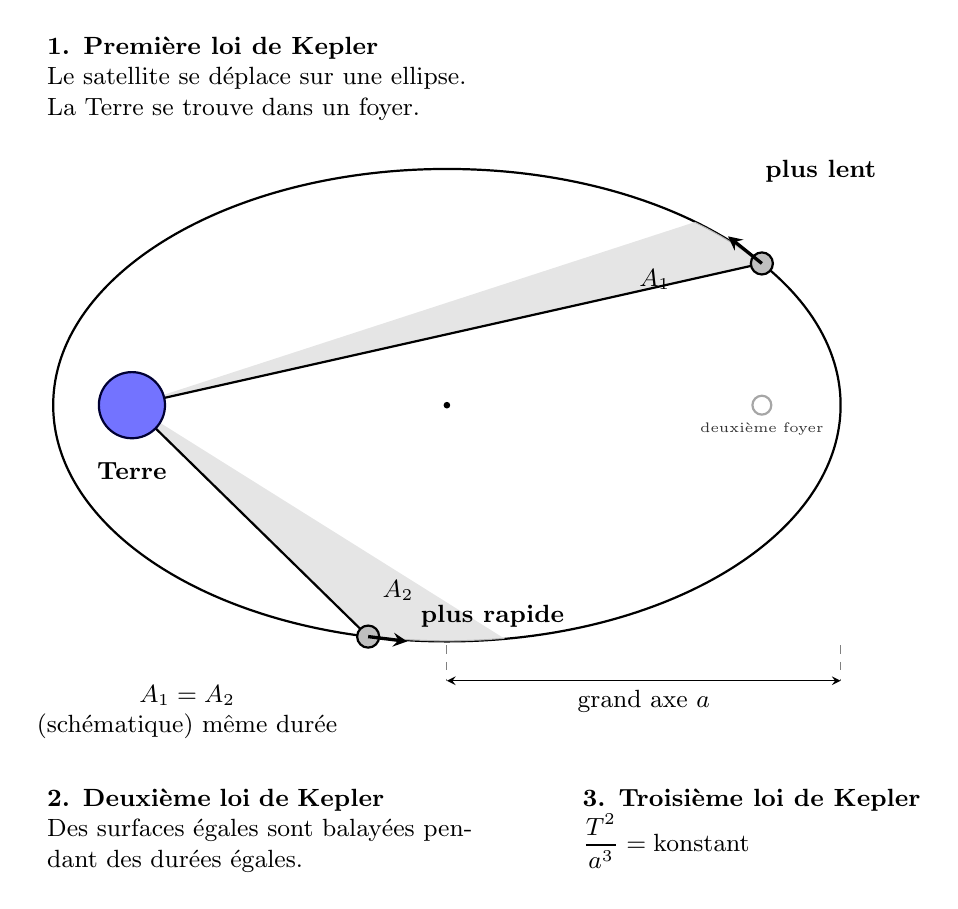
\begin{tikzpicture}[
    scale=1.0,
    >=stealth,
    every node/.style={font=\small}
]

% ============================================================
% Halbachsen  (b^2 = a^2 - c^2, hier: 3^2 = 5^2 - 4^2  -> exakt)
% ============================================================
\def\a{5}
\def\b{3}
\def\c{4}

\coordinate (Center) at (0,0);
\coordinate (Earth) at (-\c,0);
\coordinate (EmptyFocus) at (\c,0);

% ============================================================
% Ellipse
% ============================================================
\draw[thick] (Center) ellipse (\a cm and \b cm);

% ============================================================
% Überstrichene Flächen (echte elliptische Sektoren,
% Punkte entlang der Ellipse berechnet: (a cos t, b sin t))
% ============================================================

% Fläche A1 (aphelnah, kleiner Öffnungswinkel = 14°)
\fill[gray!25, opacity=0.8]
    (Earth) --
    (4.000,1.800) --
    (3.875,1.896) --
    (3.743,1.989) --
    (3.605,2.079) --
    (3.461,2.165) --
    (3.311,2.248) --
    (3.155,2.327) -- cycle;

% Fläche A2 (erdnah, grösserer Öffnungswinkel = 20°)
\fill[gray!25, opacity=0.8]
    (Earth) --
    (-1.000,-2.939) --
    (-0.714,-2.969) --
    (-0.425,-2.989) --
    (-0.134,-2.999) --
    (0.156,-2.999) --
    (0.447,-2.988) --
    (0.736,-2.967) -- cycle;

% ============================================================
% Fahrstrahlen (auf den Flächen, damit sie nicht überdeckt werden)
% ============================================================
\coordinate (S1) at (4.000,1.800);
\coordinate (S2) at (-1.000,-2.939);

\draw[thick] (Earth) -- (S1);
\draw[thick] (Earth) -- (S2);

% ============================================================
% Terre (im besetzten Brennpunkt)
% ============================================================
\filldraw[fill=blue!55, draw=blue!20!black, thick]
    (Earth) circle (0.42cm);
\node[anchor=north] at (-\c,-0.6) {\textbf{Terre}};

% Zweiter Brennpunkt (unbesetzter Brennpunkt der Ellipse)
\draw[gray!70, thick] (EmptyFocus) circle (0.12cm);
\node[below=3pt, align=center, text width=1.7cm, font=\tiny, gray!40!black]
    at (EmptyFocus) {deuxième foyer};

% Zentrum der Ellipse
\fill[black] (Center) circle (1.2pt);

% ============================================================
% Zwei Satellitenpositionen (exakt auf der Ellipse)
% ============================================================
\filldraw[fill=gray!50, draw=black, thick] (S1) circle (0.14cm);
\filldraw[fill=gray!50, draw=black, thick] (S2) circle (0.14cm);

% ============================================================
% Geschwindigkeiten (echte Bahntangenten, konsistente Umlaufrichtung;
% Pfeillänge grob proportional zur Bahngeschwindigkeit, v ~ 1/r)
% ============================================================
\draw[very thick,->] (S1) -- ++(-0.429,0.344);
\node[anchor=south west] at (3.92,2.70) {\textbf{plus lent}};

\draw[very thick,->] (S2) -- ++(0.496,-0.061)
    node[above right=1pt] {\textbf{plus rapide}};

% ============================================================
% Beschriftung der beiden Flächen
% ============================================================
\node at (2.64,1.60) {$A_1$};
\node at (-0.62,-2.35) {$A_2$};

% ============================================================
% Grosse Halbachse a  (Zentrum -> Scheitelpunkt, Länge = a,
% als Masslinie unterhalb der Ellipse mit Hilfslinien)
% ============================================================
\draw[gray, thin, dashed] (0,-3.05) -- (0,-3.5);
\draw[gray, thin, dashed] (\a,-3.05) -- (\a,-3.5);
\draw[<->,thin] (0,-3.5) -- (\a,-3.5)
    node[midway,below] {grand axe $a$};

\node[align=center] at (-3.3,-3.9)
    {$A_1=A_2$\\
     (schématique) même durée};

% ============================================================
% Keplersche Gesetze
% ============================================================
\node[align=left, anchor=west] at (-5.2,4.15)
{
\textbf{1. Première loi de Kepler}\\
Le satellite se déplace sur une ellipse.\\
La Terre se trouve dans un foyer.
};

\node[align=left, anchor=north west, text width=5.6cm] at (-5.2,-4.75)
{
\textbf{2. Deuxième loi de Kepler}\\
Des surfaces égales sont balayées pendant des durées égales.
};

\node[align=left, anchor=north west] at (1.6,-4.75)
{
\textbf{3. Troisième loi de Kepler}\\
$\displaystyle \frac{T^2}{a^3}=\mathrm{konstant}$
};

\end{tikzpicture}
